\chapter{Despliegue y validación}

El despligue de una plataforma es un paso fundamental en el desarrollo de un proyecto, ya que permite el acceso a los usuarios finales al producto final. En esta sección se describen los pasos en el despligue del frontend desarrollado con \textbf{ReactJS}. Para ello se hizo uso del servidor de \textbf{Vite}\footnote{\url{https://es.vitejs.dev/guide/}}, un servidor local de desarrollo con soporte para \textit{Typescript} y \textit{JSX} en nuestro caso.

\section{Despliegue del frontend}

\begin{enumerate}
    \item \textbf{Instalación de dependencias:} Es necesario para poder desplegar el frontend, tener instaldo \textit{Node.js}, \textit{npm}, \textit{Vite} y \textit{tailwind}.
    \item \textbf{Construcción del proyecto:} Para construir el proyecto, se debe ejecutar el comando \textit{npm run build} en la terminal.
\end{enumerate}

\section{Despliegue del backend}

El backend, que inclute la API, la base de datos y el web scrapper, se ejecutarán localmente. Para ello es necesario tener instalado \textbf{Docker} y \textbf{Docker Compose}. Para desplegar se deben ejecutar los comandos \textit{docker compose build} y \textit{docker compose up} en la terminal.

\section{GAC: Gestor Académico de Calendarios}

A continuación se mostrarán diferentes capturas (Figuras \ref{fig:GAC_inicio}, \ref{fig:GAC_menu}, \ref{fig:GAC_asignaturas}, \ref{fig:GAC_grupos}, \ref{fig:GAC_calendario}, \ref{fig:GAC_calendario_solapamientos}) de la aplicación y un enlace para un vídeo demostrativo de la misma:

\begin{figure}[H]
    \centering
    
\includegraphics[width=1\textwidth]{imagenes/GAC_inicio.png}
    \caption{Página de inicio de GAC.}
    \label{fig:GAC_inicio}
\end{figure}

\begin{figure}[H]
    \centering
    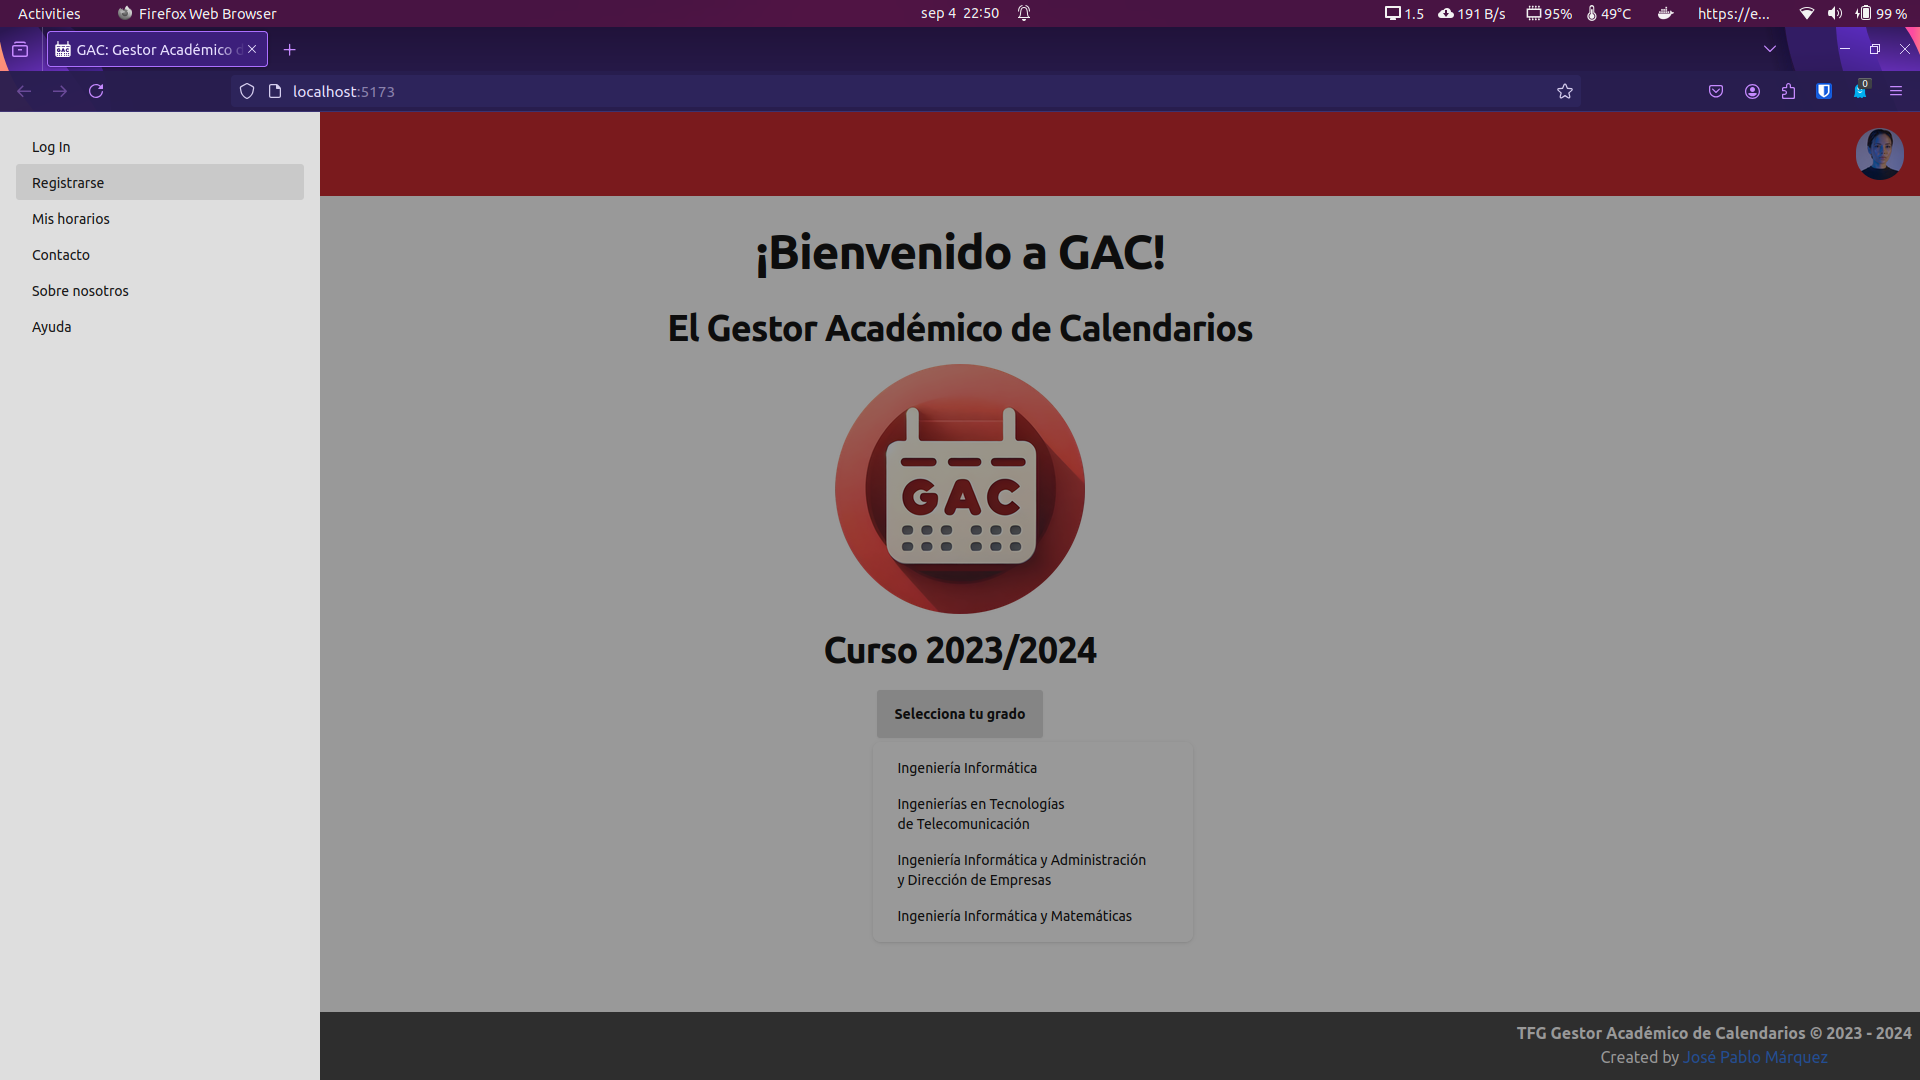
\includegraphics[width=1\textwidth]{imagenes/GAC_menu.png}
    \caption{Menú contextual de GAC.}
    \label{fig:GAC_menu}
\end{figure}

\begin{figure}[H]
    \centering
    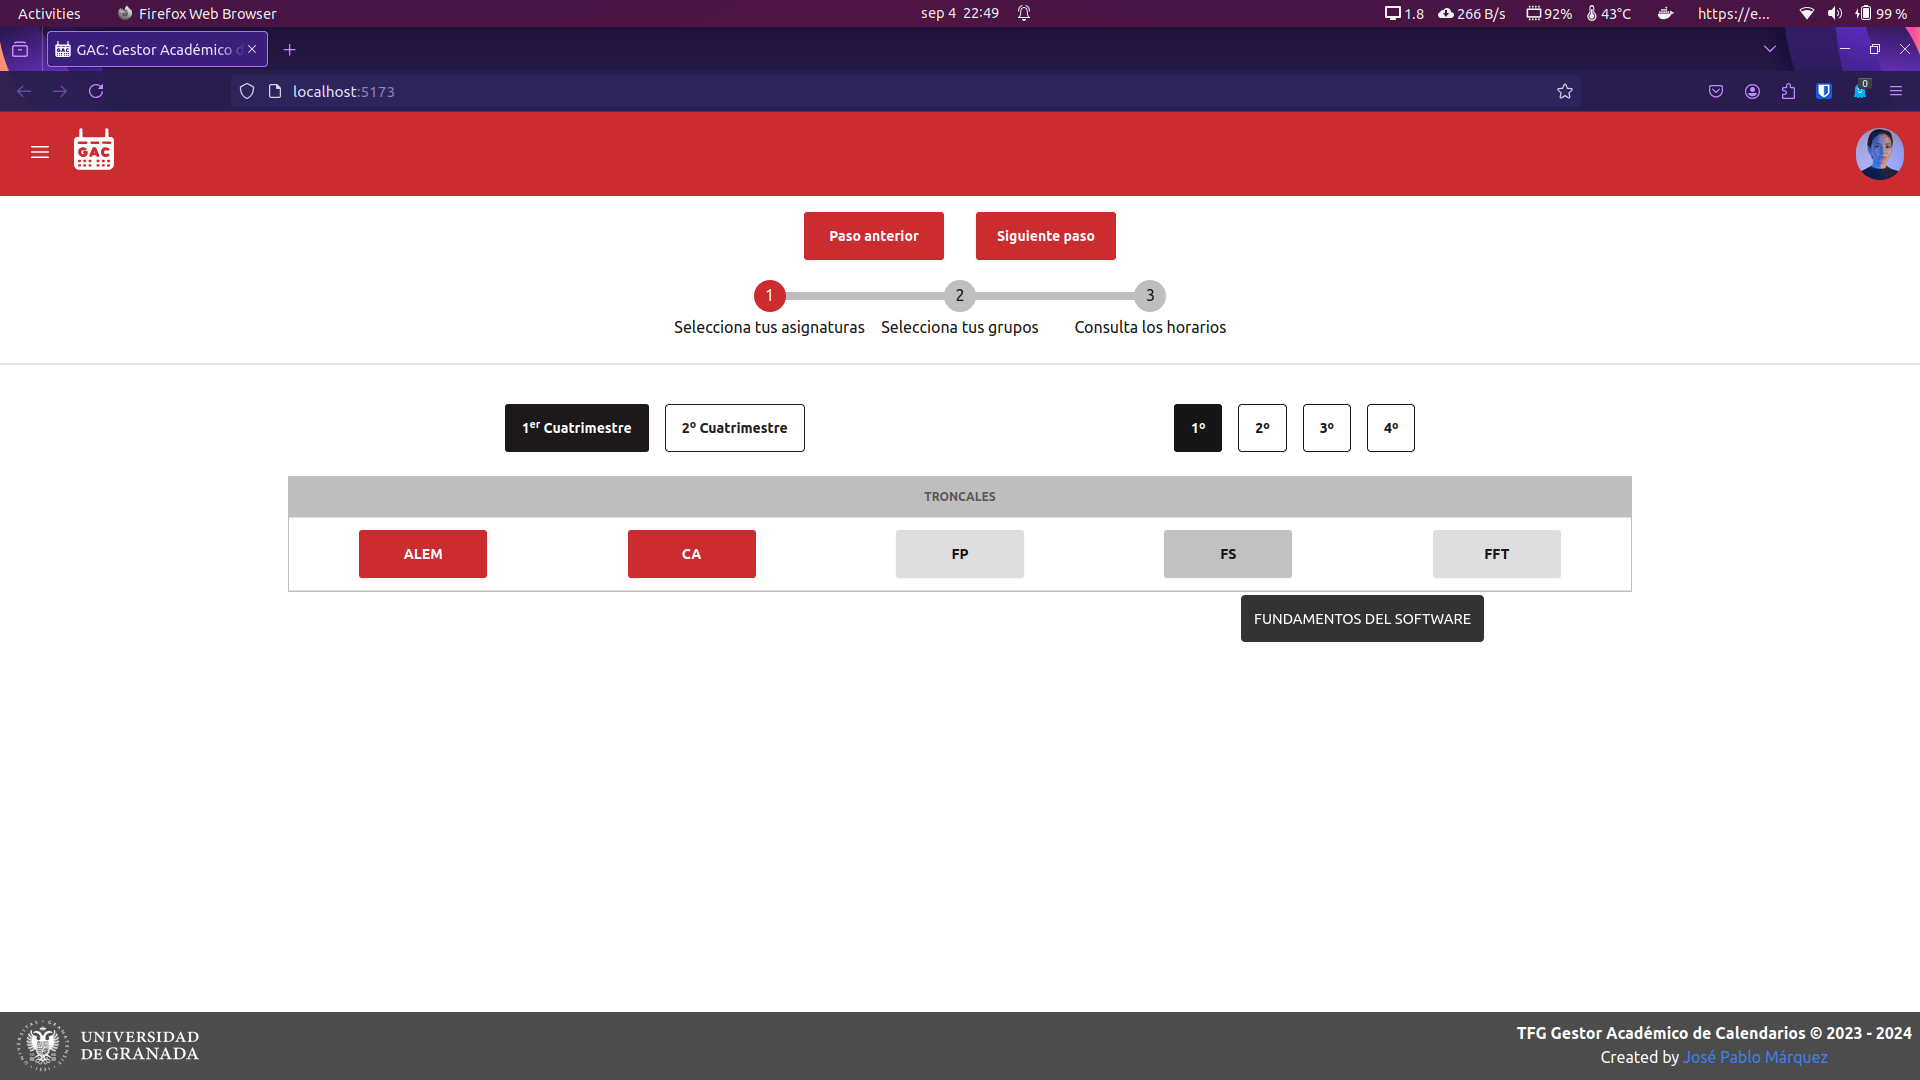
\includegraphics[width=1\textwidth]{imagenes/GAC_asignaturas.png}
    \caption{Menú de asignaturas de GAC.}
    \label{fig:GAC_asignaturas}
\end{figure}

\begin{figure}[H]
    \centering
    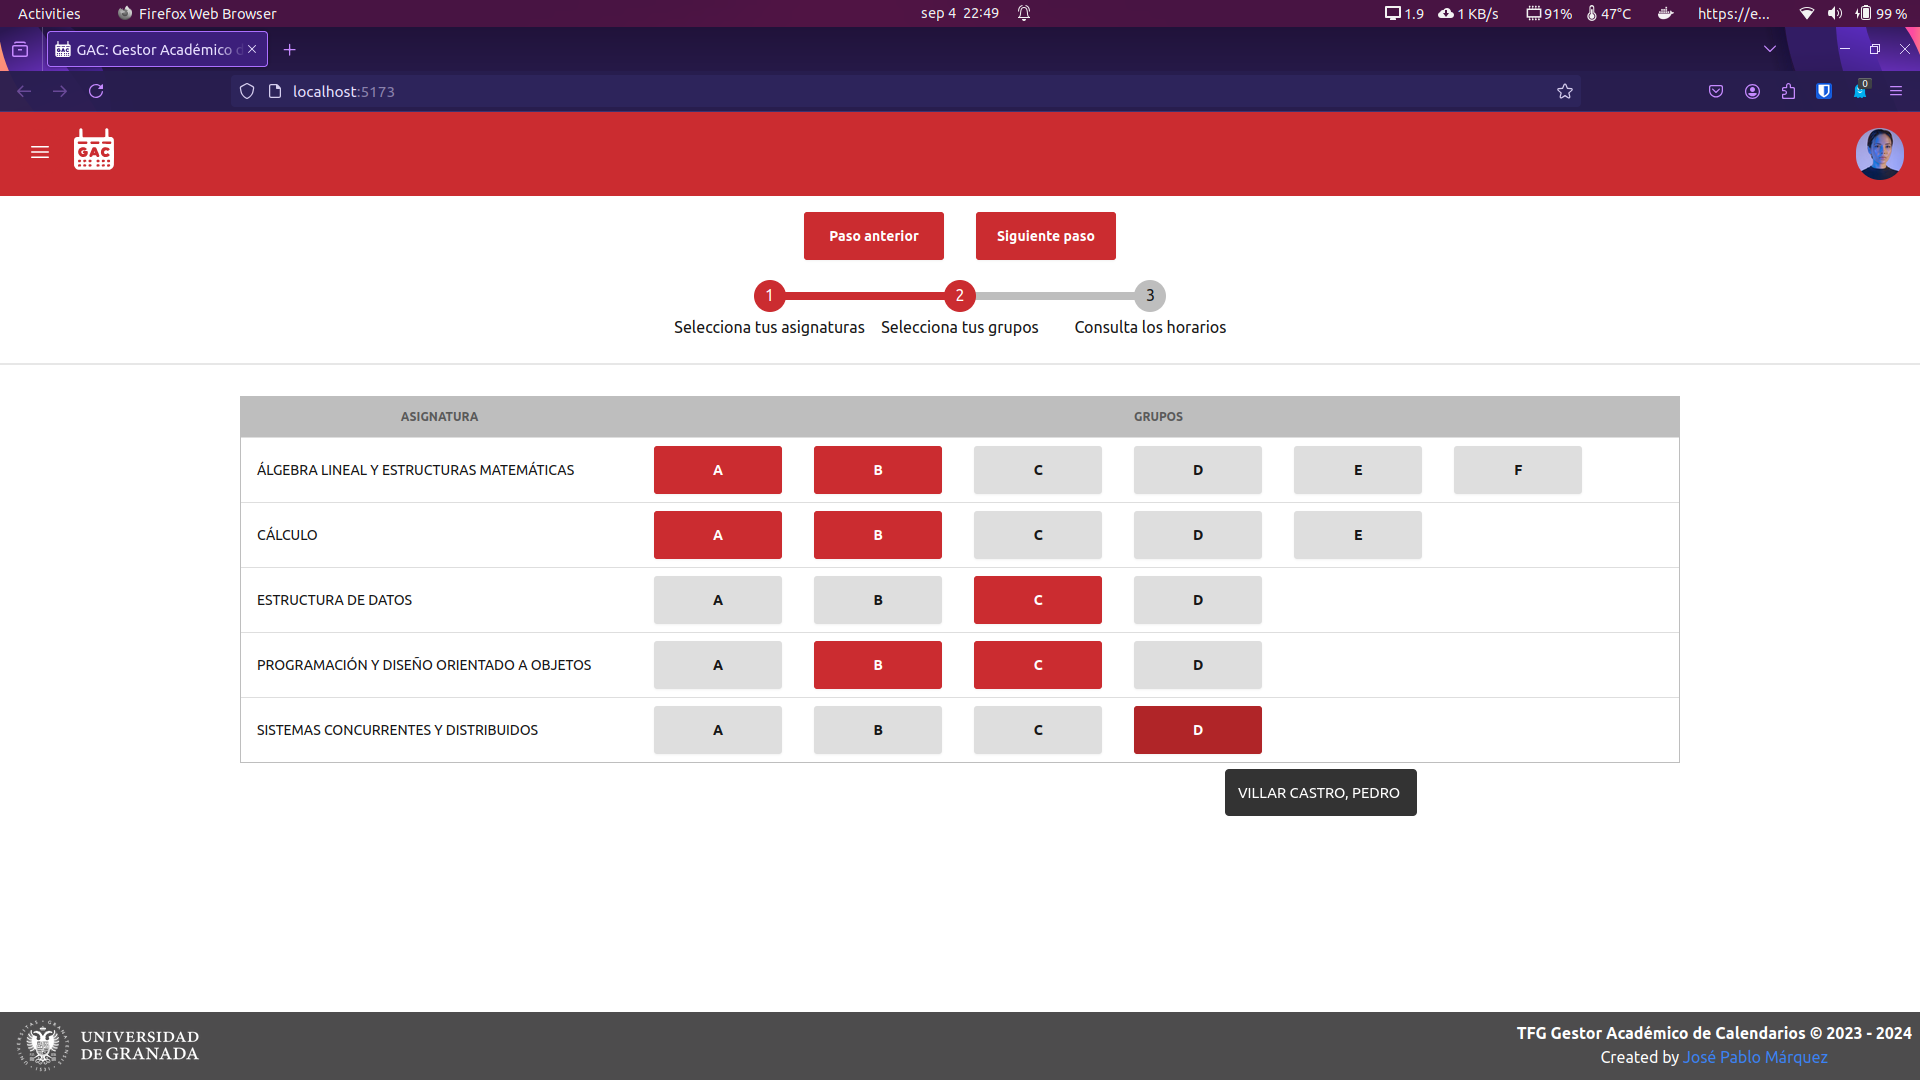
\includegraphics[width=1\textwidth]{imagenes/GAC_grupos.png}
    \caption{Menú de grupos de GAC.}
    \label{fig:GAC_grupos}
\end{figure}

\begin{figure}[H]
    \centering
    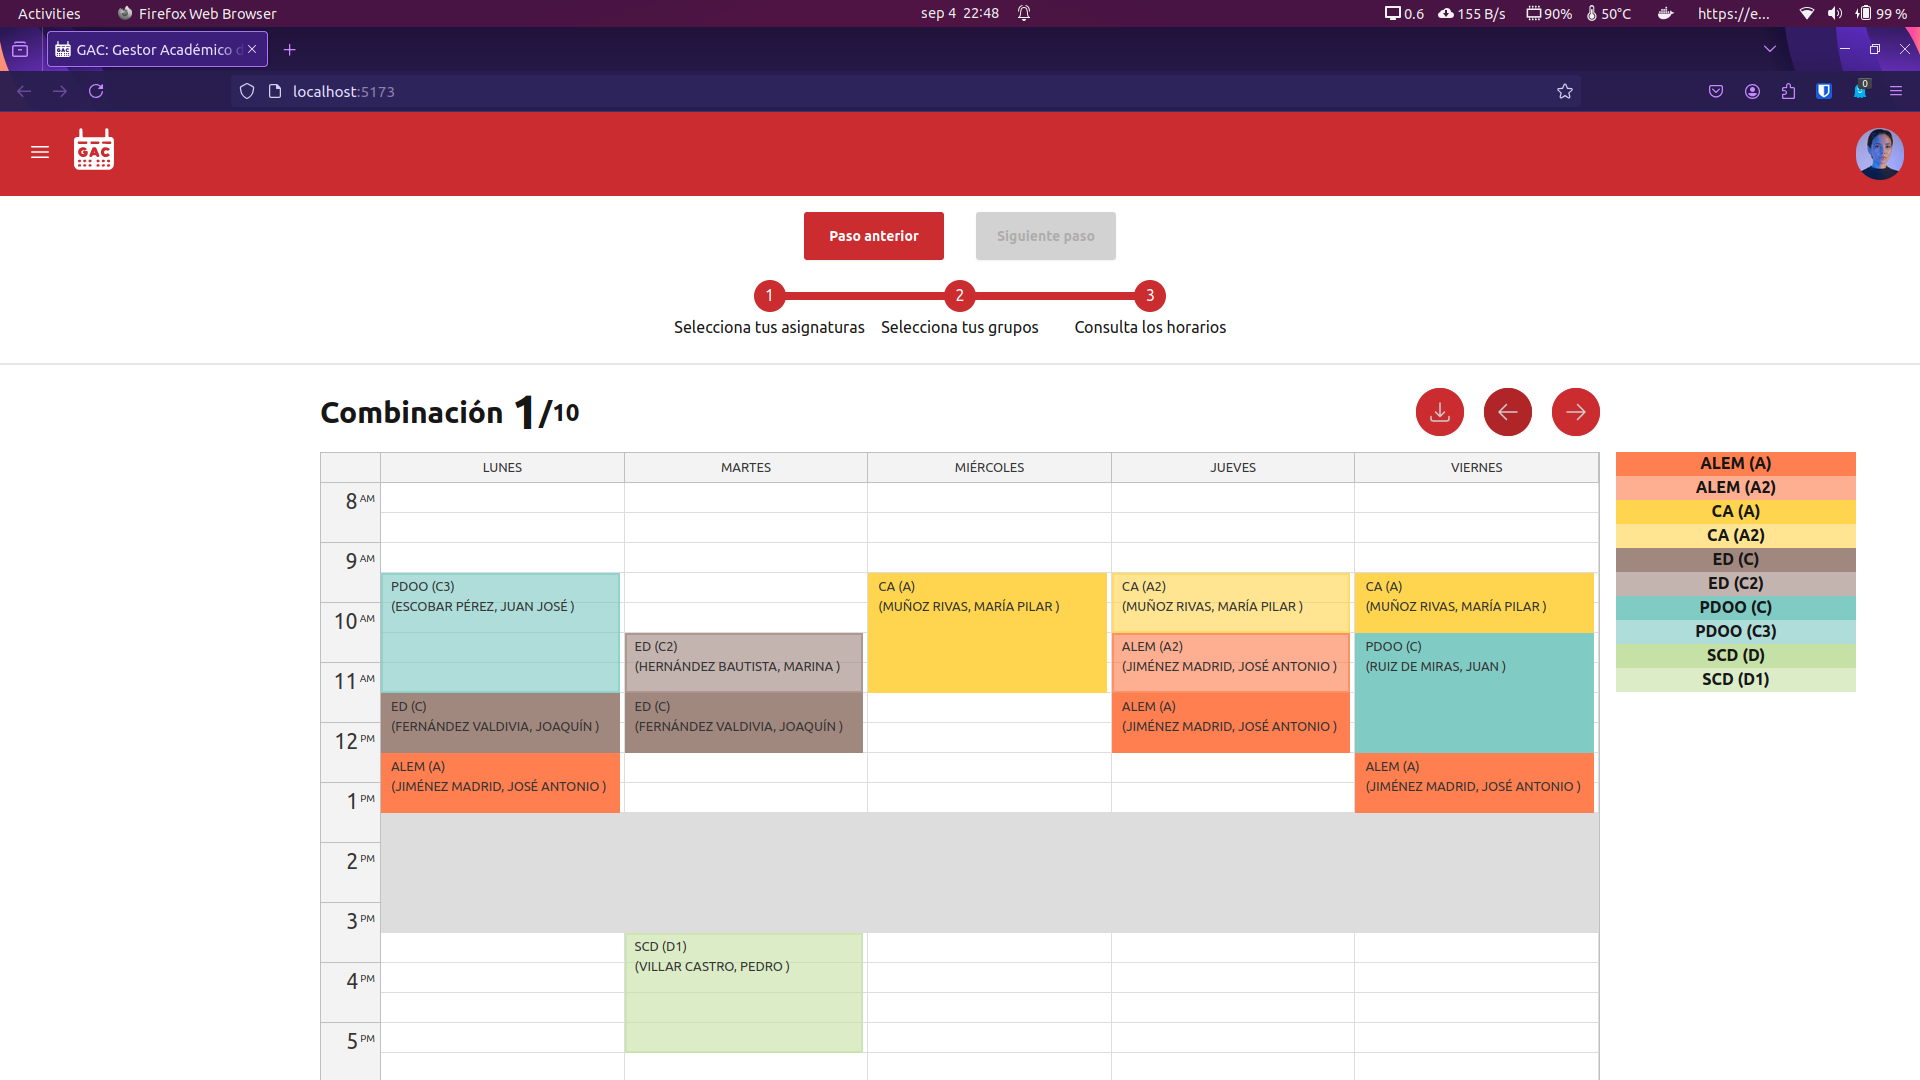
\includegraphics[width=1\textwidth]{imagenes/GAC_calendarios.png}
    \caption{Calendarios de GAC.}
    \label{fig:GAC_calendario}
\end{figure}
\vspace{3cm}
\begin{figure}[H]
    \centering
    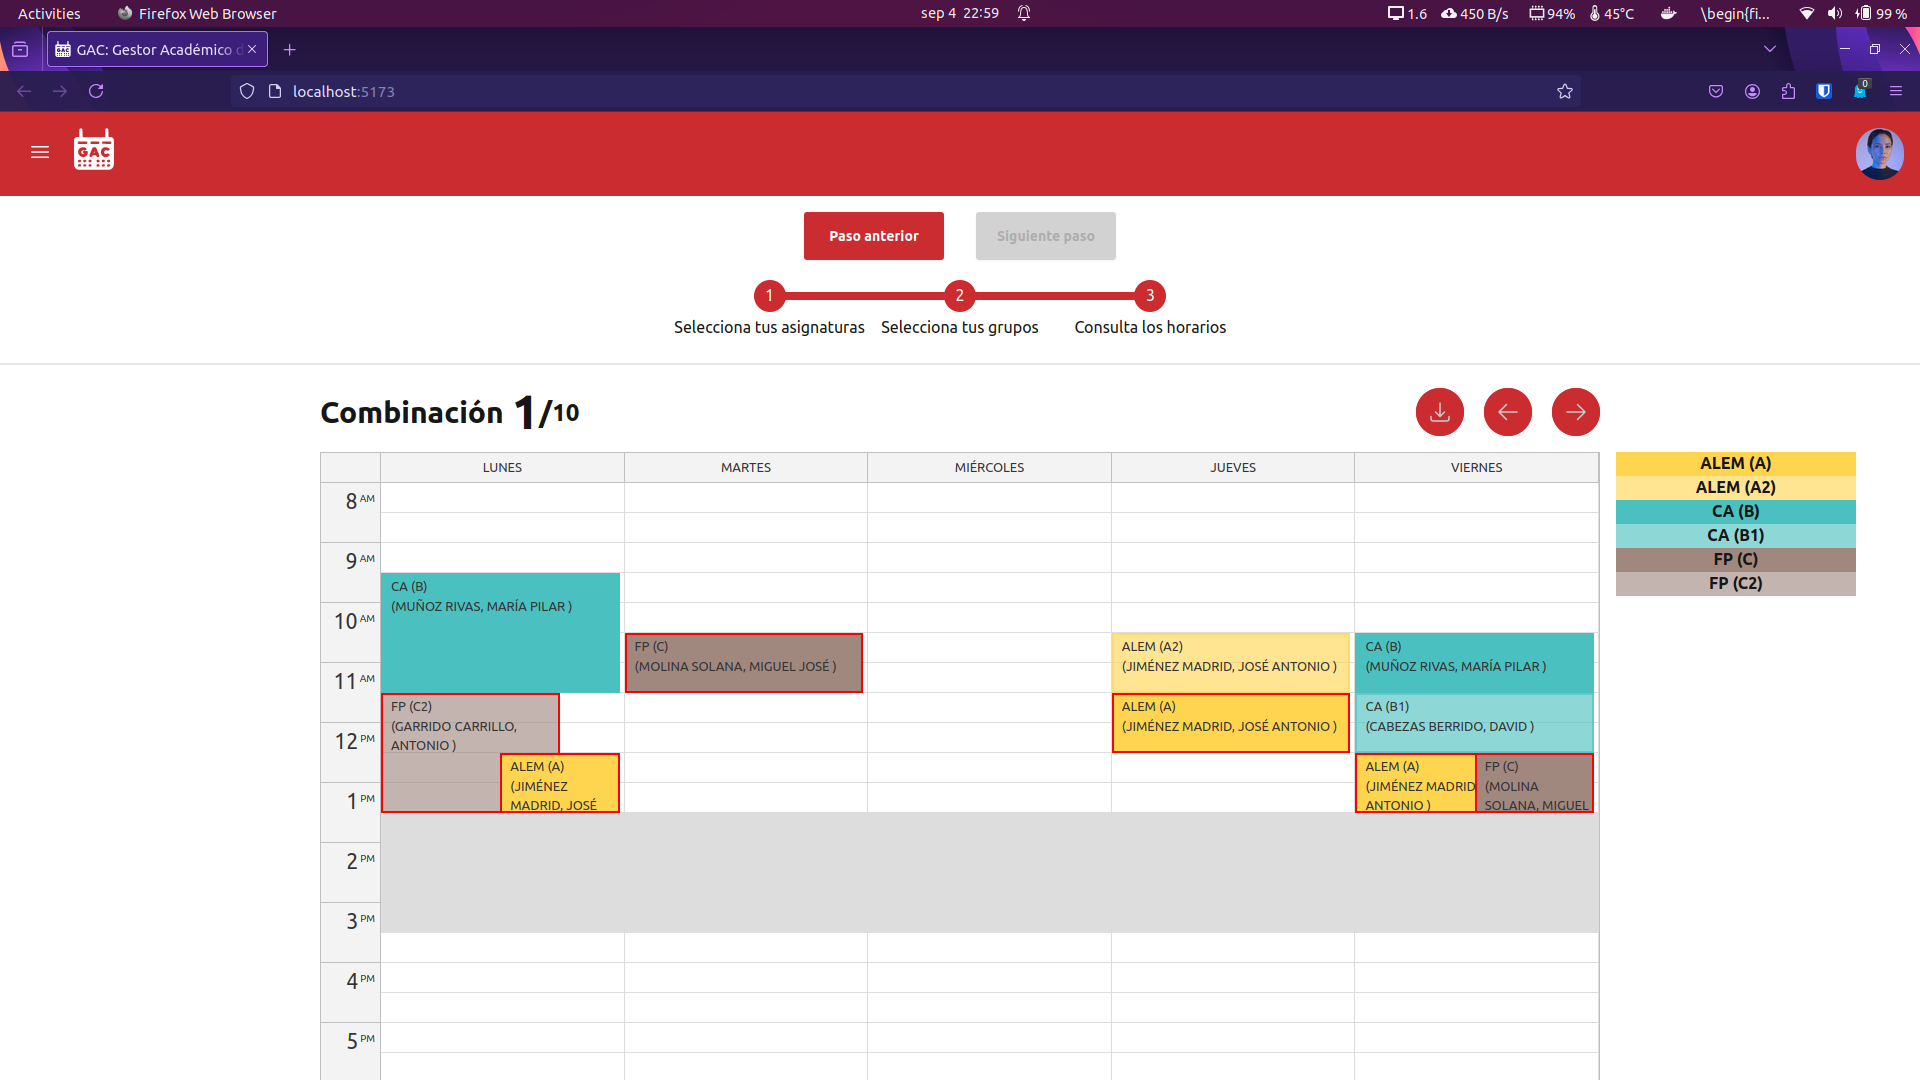
\includegraphics[width=1\textwidth]{imagenes/GAC_solapamientos.png}
    \caption{Calendarios de GAC con solapamientos destacados.}
    \label{fig:GAC_calendario_solapamientos}
\end{figure}

\subsection{Vídeo demostrativo}

A continuación hay disponible un enlace al vídeo demostrativo de la aplicación, donde se puede ver la navegación por la misma y las funcionalidades que ofrece:\newline

\url{https://youtu.be/H0-eankUrRQ}





